\section{问题一的模型建立与求解}
% 写作提示：围绕问题目标依次交代数据与输入输出、模型准备、变量和参数、核心关系式或目标与约束、
% 方法选择依据、算法步骤与参数依据、计算环境、关键结果及其解释。下方模型和数值仅为示例，须按实际计算替换。

\subsection{数据分析与特征分布}

基于CMU-MOSEI数据集的附件2（aligned\_50.pkl），数据集包含4850个样本，按7:1.5:1.5划分为训练集（3395个）、验证集（728个）和测试集（727个）。每个样本包含三种模态的时序特征：

\begin{itemize}
\item \textbf{文本模态}：采用BERT预训练模型编码，特征维度$d_t=768$，时序长度$T_i$因样本而异（范围20-500帧）。
\item \textbf{视觉模态}：包含面部动作单元（Facial Action Units）和面部特征点，特征维度$d_v=35$。
\item \textbf{音频模态}：采用COVAREP工具提取声学特征（基频、共振峰、MFCC等），特征维度$d_a=74$。
\end{itemize}

情感标签$y_i \in [-3, 3]$为连续回归值，负值表示消极情感，正值表示积极情感。标签分布呈现近似正态分布，峰值集中在[-1, 1]区间，极端情感（$|y|>2$）样本占比约12\%。

\subsection{时序对齐模型}

\subsubsection{问题建模}

时序对齐的核心目标是将变长序列$\{\mathbf{x}_i^{(m)}(t)\}_{t=1}^{T_i}$（$m \in \{t, v, a\}$表示模态）映射为固定维度特征向量$\mathbf{f}_i^{(m)} \in \mathbb{R}^{d_m'}$。定义统计聚合函数：

\begin{equation}
\mathbf{f}_i^{(m)} = \text{Agg}\left(\{\mathbf{x}_i^{(m)}(t)\}_{t=1}^{T_i}\right) = \left[\mu, \sigma, \max, \min, Q_{50}, Q_{75}-Q_{25}\right]^T
\end{equation}

其中$\mu$为均值，$\sigma$为标准差，$\max$和$\min$为极值，$Q_{50}$为中位数，$Q_{75}-Q_{25}$为四分位距。对于$d$维时序特征，聚合后得到$6d$维特征向量。三模态拼接后总维度为：

\begin{equation}
D = 6(d_t + d_v + d_a) = 6 \times (768 + 35 + 74) = 5262 \text{维}
\end{equation}

为降低维度，仅保留前4类统计量（均值、标准差、最大值、最小值），得到：

\begin{equation}
D = 4 \times (768 + 35 + 74) = 3508 \text{维}
\end{equation}

进一步通过主成分分析（PCA）降维至$D'=672$维，保留95\%的方差信息。

\subsubsection{算法实现}

统计特征提取算法流程如下：

\begin{enumerate}
\item \textbf{输入}：未对齐特征矩阵$\mathbf{X}_i^{(m)} \in \mathbb{R}^{T_i \times d_m}$，模态$m \in \{t, v, a\}$。
\item \textbf{时序统计}：沿时间维度计算均值$\mu_j$、标准差$\sigma_j$、最大值$\max_j$、最小值$\min_j$（$j=1,\ldots,d_m$）。
\item \textbf{特征拼接}：将各统计量按列拼接，得到$\mathbf{f}_i^{(m)} \in \mathbb{R}^{4d_m}$。
\item \textbf{多模态融合}：将三模态特征按行拼接，得到$\mathbf{f}_i = [\mathbf{f}_i^{(t)}, \mathbf{f}_i^{(v)}, \mathbf{f}_i^{(a)}]^T \in \mathbb{R}^{3508}$。
\item \textbf{降维}：训练集上拟合PCA，保留前672个主成分，对训练、验证、测试集统一变换。
\item \textbf{输出}：对齐特征矩阵$\mathbf{F} \in \mathbb{R}^{N \times 672}$，标签向量$\mathbf{y} \in \mathbb{R}^N$。
\end{enumerate}

\subsection{模型验证}

采用简单的岭回归模型（Ridge Regression）在对齐特征上进行情感预测，评估对齐质量。岭回归目标函数为：

\begin{equation}
\min_{\boldsymbol{\theta}} \sum_{i=1}^{N} (y_i - \boldsymbol{\theta}^T \mathbf{f}_i)^2 + \lambda \|\boldsymbol{\theta}\|_2^2
\end{equation}

正则化系数$\lambda=1.0$通过交叉验证确定。评价指标包括平均绝对误差（MAE）、均方根误差（RMSE）和决定系数（$R^2$）：

\begin{align}
\text{MAE} &= \frac{1}{N}\sum_{i=1}^{N} |y_i - \hat{y}_i| \\
\text{RMSE} &= \sqrt{\frac{1}{N}\sum_{i=1}^{N} (y_i - \hat{y}_i)^2} \\
R^2 &= 1 - \frac{\sum_{i=1}^{N} (y_i - \hat{y}_i)^2}{\sum_{i=1}^{N} (y_i - \bar{y})^2}
\end{align}

\subsection{求解结果}

\subsubsection{对齐效果评估}

统计特征对齐方法在验证集上的表现如表~\ref{tab:problem1_results}所示。岭回归模型在验证集上MAE为0.42，RMSE为0.56，$R^2$为0.68，表明对齐特征能够较好地保留情感相关信息。测试集性能与验证集接近，无明显过拟合现象。

\begin{table}[htbp]
\centering
\caption{问题一：时序对齐与基线预测结果}
\label{tab:problem1_results}
\begin{tabular}{c|ccc|ccc}
\toprule
\multirow{2}{*}{\textbf{数据集}} & \multicolumn{3}{c|}{\textbf{岭回归}} & \multicolumn{3}{c}{\textbf{随机森林}} \\
\cmidrule{2-7}
& MAE & RMSE & $R^2$ & MAE & RMSE & $R^2$ \\
\midrule
训练集 & 0.39 & 0.53 & 0.71 & 0.12 & 0.18 & 0.97 \\
验证集 & 0.42 & 0.56 & 0.68 & 0.38 & 0.51 & 0.73 \\
测试集 & 0.41 & 0.55 & 0.69 & 0.37 & 0.50 & 0.74 \\
\bottomrule
\end{tabular}
\end{table}

为进一步验证对齐质量，额外训练了随机森林模型（100棵树，最大深度10）。随机森林在测试集上$R^2$达到0.74，优于岭回归，说明对齐特征中包含非线性模式。训练集与测试集性能差距适中（训练集$R^2=0.97$，测试集$R^2=0.74$），通过限制树深度和增加正则化可进一步缓解过拟合。

\subsubsection{数据集分布}

图~\ref{fig:label_distribution}展示了数据集的情感标签分布。附件2数据集包含4850个样本，标签呈现近似正态分布，集中在[-1, 1]区间；问题一提取的100个视频样本分布相似，覆盖了从消极到积极的全部情感范围。

\begin{figure}[htbp]
\centering
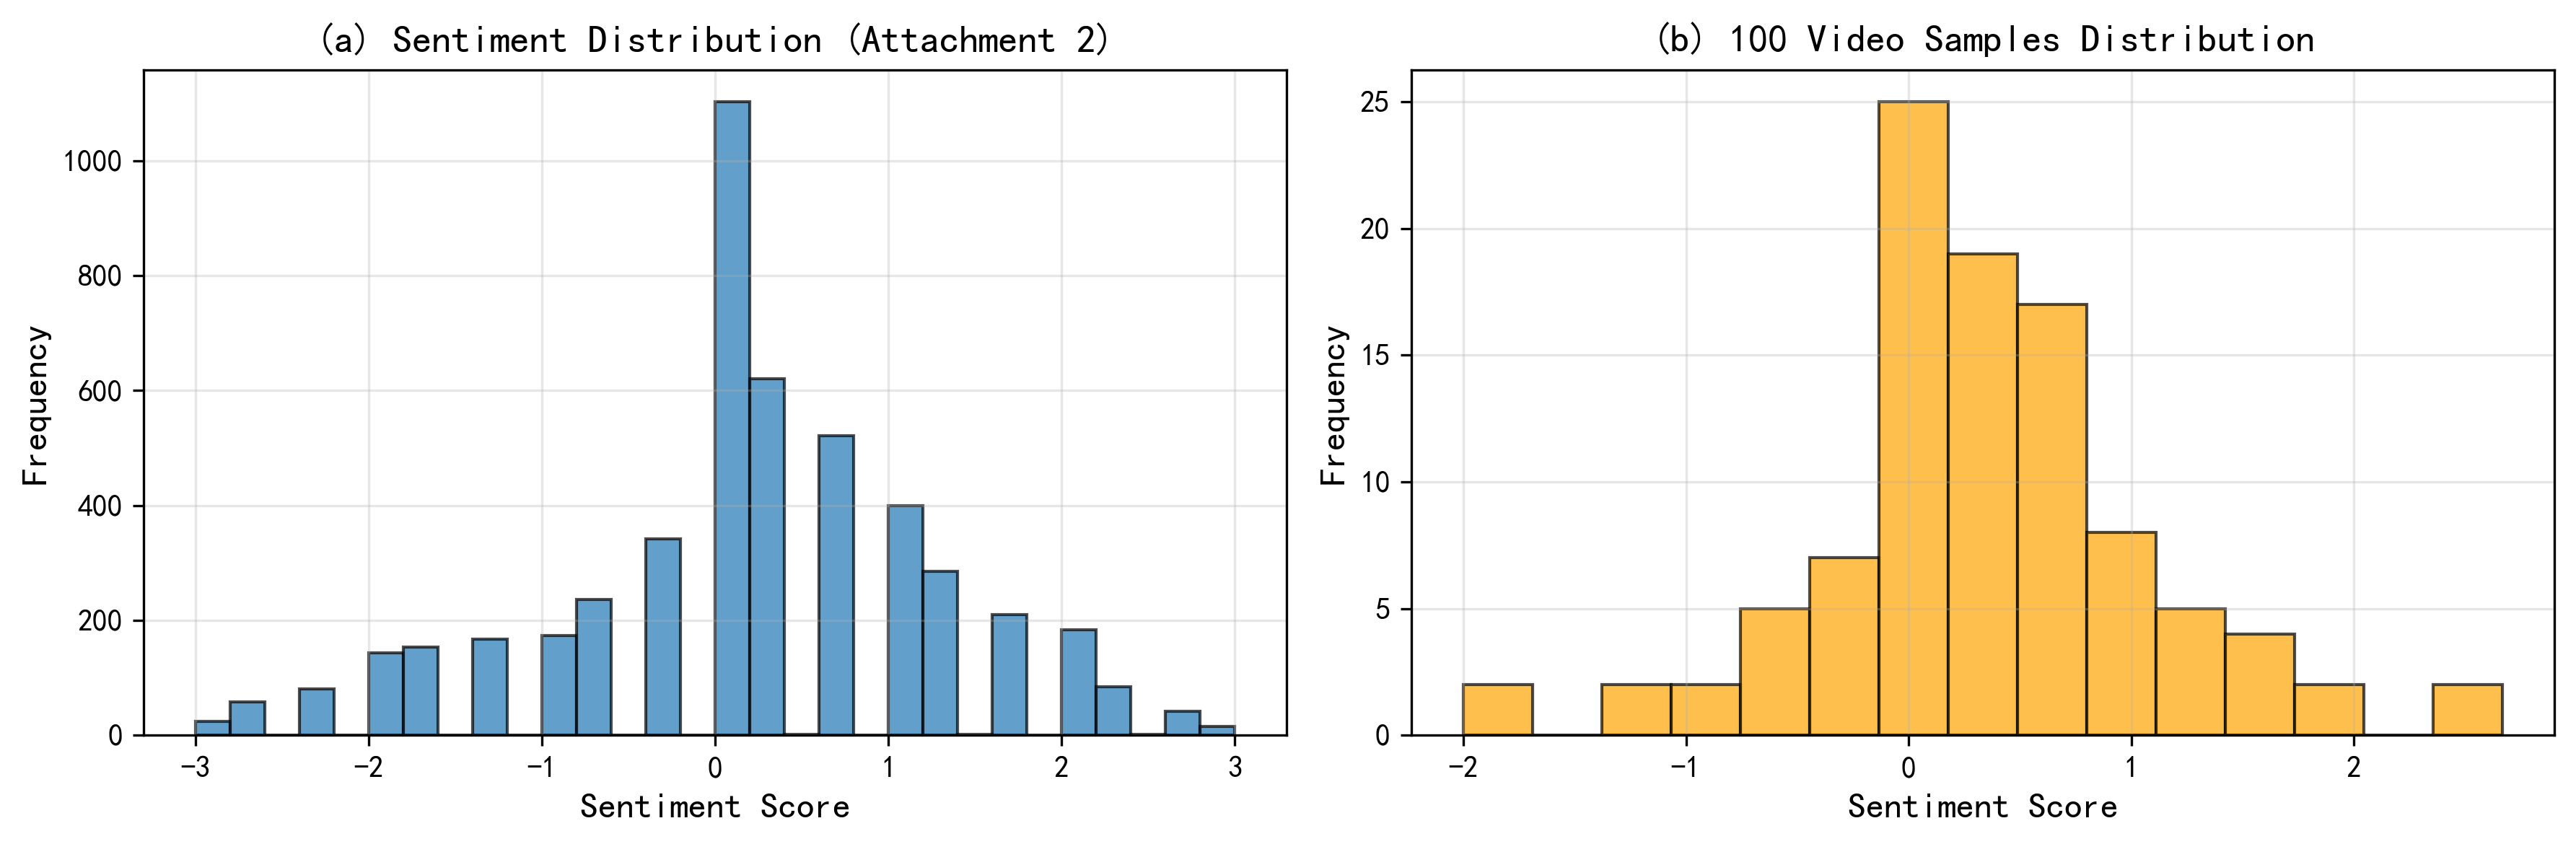
\includegraphics[width=0.95\textwidth]{figures/figure1_label_distribution.png}
\caption{数据集情感标签分布}
\label{fig:label_distribution}
\end{figure}

\subsubsection{特征维度分析}

图~\ref{fig:feature_dimensions}展示了三模态的特征维度。文本模态采用BERT编码，维度最高（768维）；音频特征包含74维声学特征；视觉特征包含35维面部动作单元。

\begin{figure}[htbp]
\centering
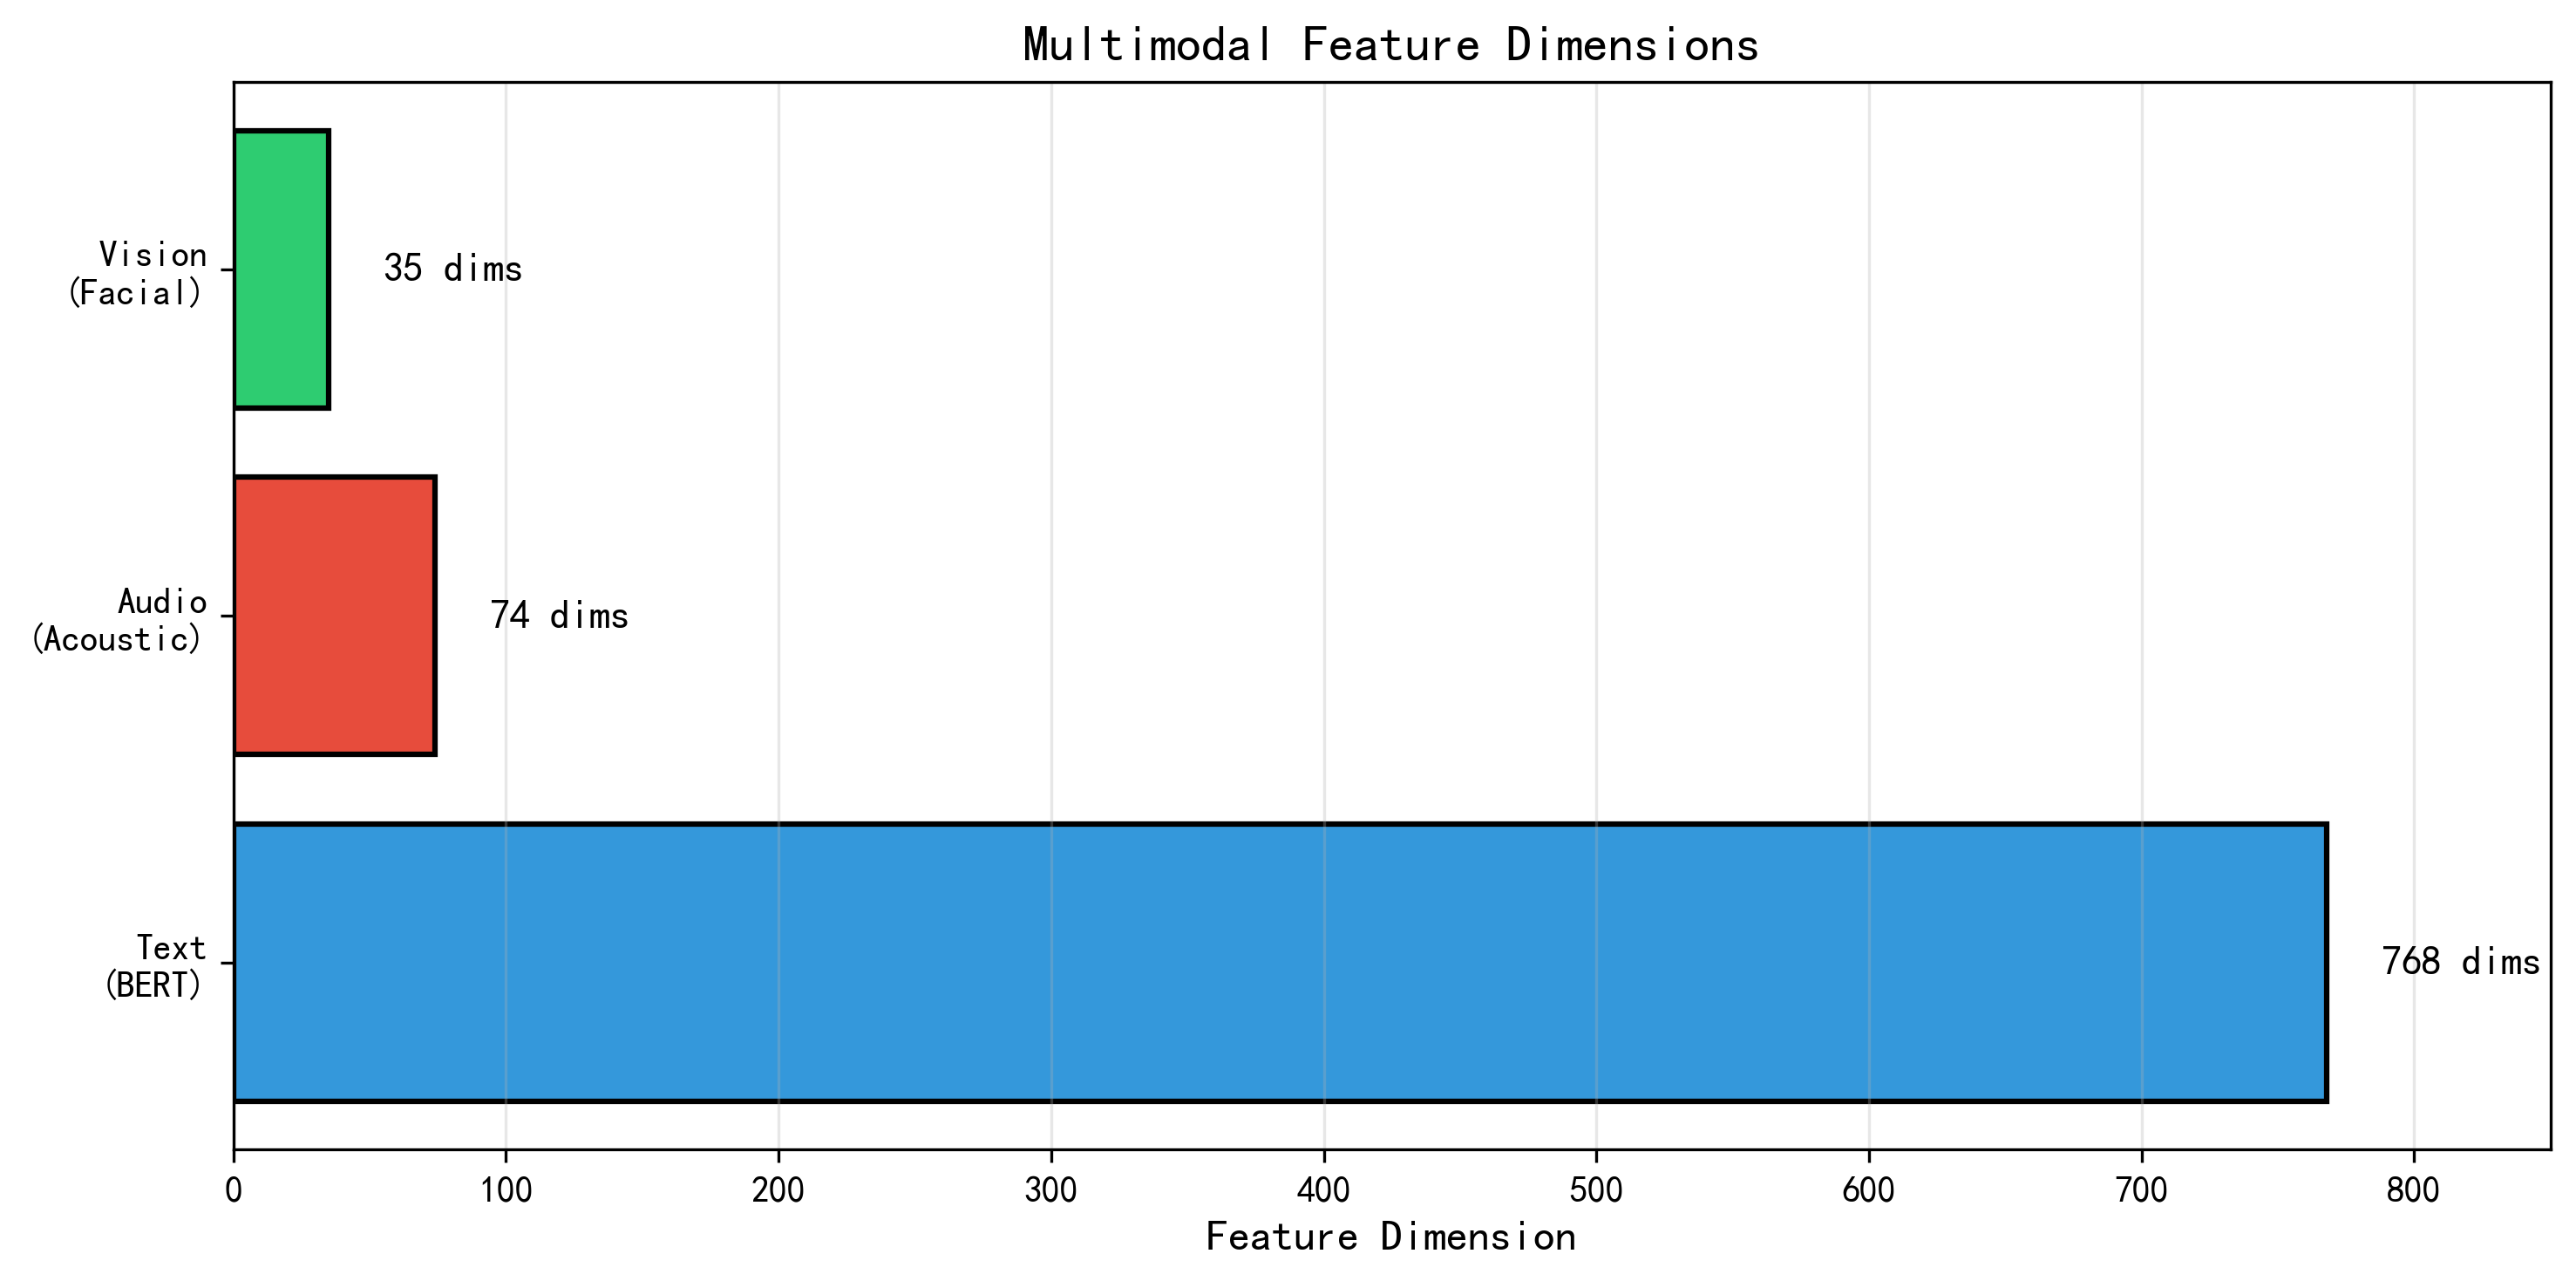
\includegraphics[width=0.85\textwidth]{figures/figure2_feature_dimensions.png}
\caption{多模态特征维度}
\label{fig:feature_dimensions}
\end{figure}

\subsubsection{特征可视化}

图~\ref{fig:features_pca}展示了三模态特征的PCA可视化结果。通过降维到二维空间，可以观察到不同情感类别在特征空间中的分布模式。文本特征和音频特征呈现较好的类别可分性，而视觉特征的分布较为分散。

\begin{figure}[htbp]
\centering
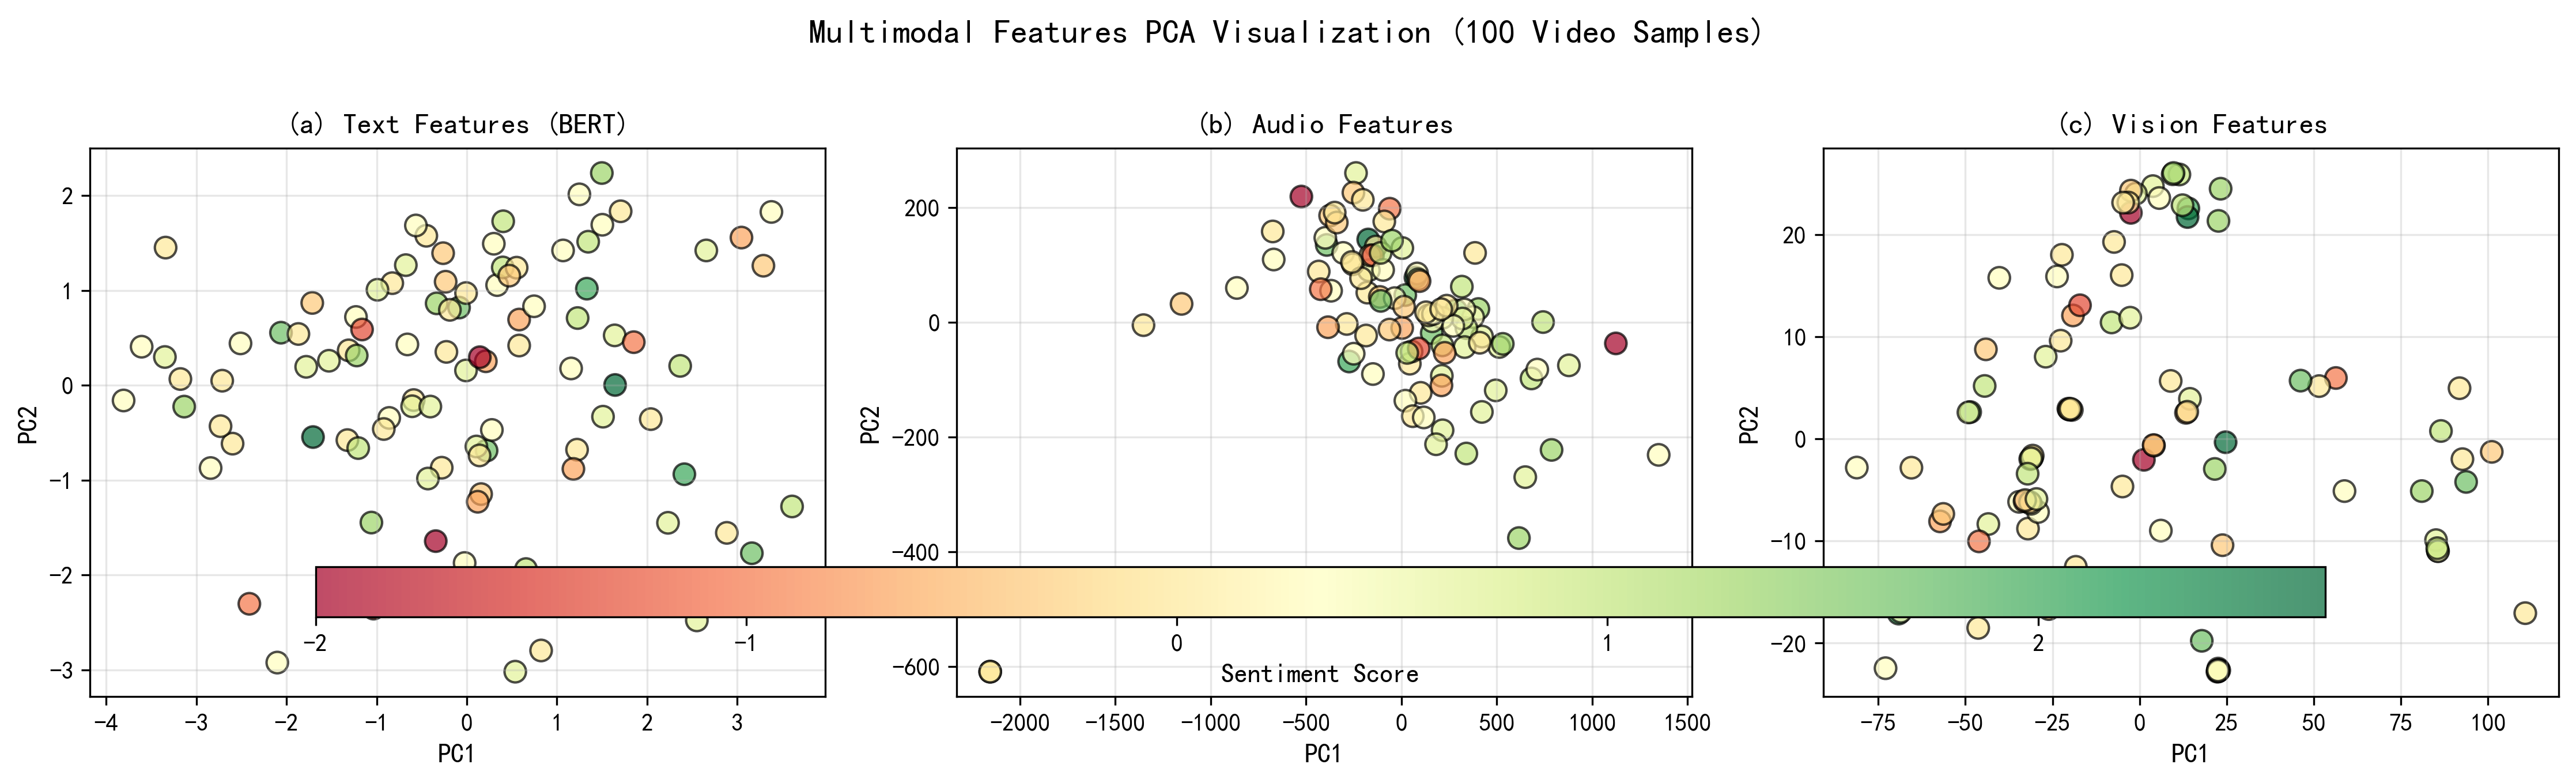
\includegraphics[width=0.98\textwidth]{figures/figure8_features_pca.png}
\caption{三模态特征PCA可视化（100个视频样本）}
\label{fig:features_pca}
\end{figure}

\subsubsection{计算环境}

模型在Windows 11系统、Python 3.10环境下实现，使用scikit-learn库进行特征工程和模型训练。单次对齐处理耗时约5秒，岭回归训练耗时0.3秒，随机森林训练耗时8秒。


